\chapter{Metrics hyperparameter tuning}

After taking the best possible loss minimizing ERM and tuning the parameters we want to have something humans readable so we use metrics that are measure of quality of our choice.
The evaluation of supervised Machine learning are different:
\begin{enumerate}
    \item efficiency
    \item scalability
    \item robustness
    \item interpretability
\end{enumerate}

The quality of the prediction is different from the prediction one, there are:
\begin{enumerate}
    \item Confusion matrix
    \item Accuracy 
    \item Precision 
    \item ROC curve
\end{enumerate}
\subsection{Confusion matrix}
\begin{figure}[H]
    \centering
    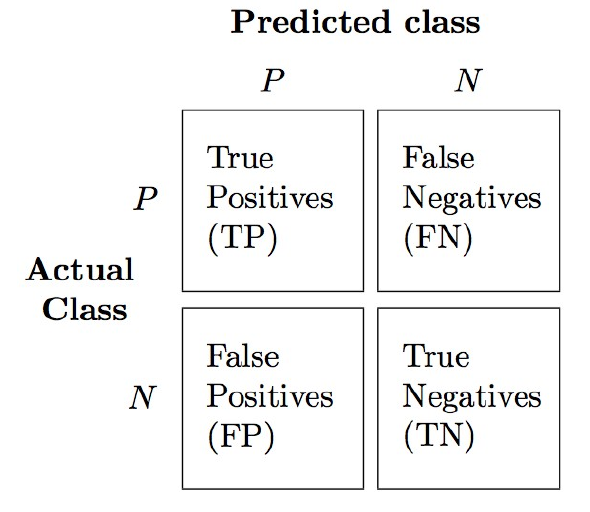
\includegraphics[scale=0.3]{images/PM/PM1.png}
    \caption{Example of confusion matrix for binary classifier}
    \label{fig:enter-label}
\end{figure}

\subsection{Accuracy}
It is the most widely-used metric for model evaluation: $acc = \dfrac{\text{Number of correctly classified obj}}{\text{Number of classified obj}}$ and for binary classifiers became : 
$ Accuracy = \dfrac{\text{TP + TN}}{\text{TP + TN + FP + FN}}$. The one related to 0/1 loss is: $ 1- (1/m) \sum\limits_{i=1}^m L((x^{(i)}, y^{(i)}),h) $.

Accuracy might be misleading when we have not balanced samples and maybe a missclassification for some objects of a given class could have different importance like in medical problem. For this problem we can use other correlated measure like \textbf{precision}:
$ p = \dfrac{\text{Number of objects correctly assigned to c}}{\text{Number of objects assigned to c}}$ or $ p = \dfrac{TP}{TP+FP}$ 

and the \textbf{recall}:
$ \dfrac{\text{Number of objects correctly assigned to c}}{\text{Number of objects belonging to c}}$ or $ r = \dfrac{TP}{TP+FN}$. Precision measure how many selected items are relevant and the recall measure how many relevant items are selected; both are measure applied to \textbf{every class}. Combining them we can have F-measure: $F = \dfrac{2rp}{r+p} $ or $F=\dfrac{2TP}{2TP + FP +FN}$ that is the harmonic mean.

\subsection{ROC curve}
ROC (Receiver Operating Characteristics) developed for noisy signals to find the trade-off between positive hits and false alarms.

\begin{figure}[H]
    \centering
    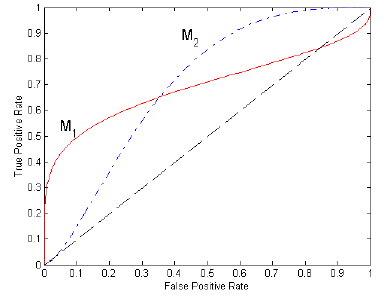
\includegraphics[scale=0.6]{images/PM/PM2.png}
    \caption{ROC curve, each point is a different Hypothesis. Ideally we want to stay in the top left corner but we can't so we have to choose the trade-off as humans}
    \label{fig:enter-label}
\end{figure}

Normally we choose the one with more area under the function (integral) if we don't have constraint. This is called AUC ROC curve.


\section{Learning curve}